% document formatting
\documentclass[10pt]{article}
\usepackage[utf8]{inputenc}
\usepackage[left=1in,right=1in,top=1in,bottom=1in]{geometry}
\usepackage[T1]{fontenc}
\usepackage{xcolor}

% math symbols, etc.
\usepackage{amsmath, amsfonts, amssymb, amsthm}
\usepackage{dsfont}

% lists
\usepackage{enumerate, enumitem}
\usepackage{tabularx}

% images
\usepackage{graphicx} % for images
\usepackage{tikz}

% code blocks
% \usepackage{minted, listings} 

% verbatim greek
\usepackage{alphabeta}

\graphicspath{{./assets/images/Module 4}}

\title{02-680 Module 4 \\ \large{Essentials of Mathematics and Statistics}}
 
\author{Aidan Jan}

\date{\today}

\begin{document}
\maketitle

\section*{Graphs}
\textbf{Graphs} are powerful tools for modeling structured \textbf{relationships} between entities.  A graph consists of:
\begin{itemize}
	\item \textbf{Nodes} (or Vertices): The entities in the graph
	\item \textbf{Edges} (or Links): The relationships between pairs of nodes.
\end{itemize}
A graph is also called a \textbf{network}.

\subsection*{Undirected Graphs}
\begin{itemize}
	\item In \textbf{undirected graphs}, edges represent mutual relationships.  If node $A$ is connected to node $B$, then node $B$ is also connected to node $A$.
\end{itemize}
Many real-world relationships are mutual.  This representation is suitable for systems where all connections are peer-to-peer.

\subsection*{Directed Graphical Models}
In a social network, each \textbf{node} represents a person, and each \textbf{directed edge} represents a relationship such as following, influencing, or messaging.  These directed connections capture how information, behavior, or influence propagates across the network.

\subsection*{Directed Graph vs. Undirected Graph}
In a directed graph, an edge is an \textbf{ordered pair} of vertices ("an edge from $u$ to $v$") and in an undirected graph, an edge is an unordered pair of vertices ("an edge between $u$ and $v$").
\begin{center} 
	\includegraphics*[width=0.7\textwidth]{M4_1.png} 
\end{center}
\rule{\textwidth}{0.4pt}
\par
\pagebreak
A \textbf{graph} is a mathematical structure used to model pairwise relationships.  We typically write a graph as a tuple $G = \langle V, E \rangle$.
\begin{itemize}
	\item $V$ is a set of nodes or vertices
	\item $E$ is a set of edges, each connecting a pair of nodes.
	\begin{itemize}
	    \item $E \subseteq V \times V$ if $G$ is \textbf{directed}
	    \item $E \subseteq \{\{u, v\} \::\: u, v \in V\}$ if $G$ is \textbf{undirected}
	    \item Note that one edge can loop around the same node.  (e.g., $u = v$)
    \end{itemize}
\end{itemize}
Nodes in a graph are typically drawn as circles ad edges are represented as lines.  In directed graphs, each edge is drawn with an arrow indicating its orientation ("which way it goes").

\subsection*{Parents and Children}
In a directed graph, there exists the notion of parent nodes and child nodes.  If an arrow connects two variables $X$ and $Y$ (in either direction) we say that $X$ and $Y$ are adjacent.  If there is an arrow from $X$ to $Y$, then $X$ is a parent of $Y$, and $Y$ is a child of $X$.  A \textbf{directed path} between two variables is a set of arrows all pointing in the same direction linking one variable to the other such as:
\begin{center} 
	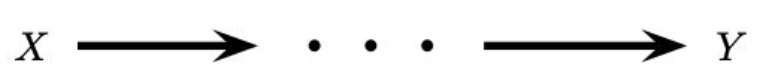
\includegraphics[width=0.6\textwidth]{M4_2.png}
\end{center}

\subsection*{Some Examples of Graphs}
To understand a \textbf{directed graph}, think about the difference between:
\begin{itemize}
	\item Twitter follows: $A \rightarrow B$ (directed)
	\item Facebook friendships: $A - B$ (undirected)
\end{itemize}
\begin{center} 
	\includegraphics*[width=0.9\textwidth]{M4_3.png} 
\end{center}

\subsection*{Path in a Directed Graph}
Some examples of things that can be represented as \textbf{graphs}: train/flight maps, cell interactions, social networks, etc.  A \textbf{path} is a sequence of nodes:
\[\langle v_1, v_2, v_3, \dots, v_k \rangle\]
\begin{center}
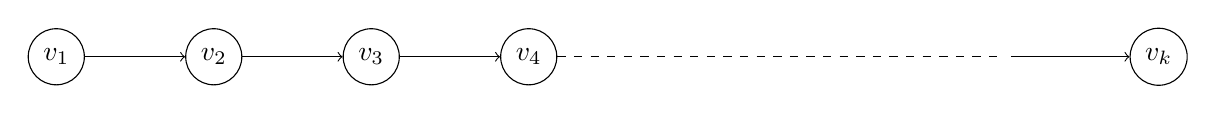
\begin{tikzpicture}
    \node[draw, circle] at (0, 0) (1) {$v_1$};
    \node[draw, circle] at (2, 0) (2) {$v_2$};
    \node[draw, circle] at (4, 0) (3) {$v_3$};
    \node[draw, circle] at (6, 0) (4) {$v_4$};
    \node at (12, 0) (dots) {};
    \node[draw, circle] at (14, 0) (k) {$v_k$};
    \draw[->] (1) edge (2);
    \draw[->] (2) edge (3);
    \draw[->] (3) edge (4);
    \draw[dashed] (4) edge (12, 0);
    \draw[->] (dots) edge (k);
\end{tikzpicture}
\end{center}
\begin{itemize}
	\item $\langle v_i, v_{i + 1} \rangle \in E$ if $G$ is \textbf{directed}
	\item $\{v_1, v_{i + 1}\} \in E$ if $G$ is \textbf{undirected}
\end{itemize}
We say that the \textbf{path} has length $k$, and that a path is from $v_1$ to $v_k$.

\subsection*{Route Graph}
In the case of a route graph (e.g., for navigation or delivery), each edge might be labeled with a street name (a string), but in other types of graphs the labels could be numerical values (such as distance, time, or cost) - which we usually call \textbf{weights}.\\
\begin{itemize}
	\item A \textbf{path label} could be the concatenation of street names (e.g. "Main St." \textrightarrow "Broadway" \textrightarrow "5th Ave.")
	\item A \textbf{path weight} could be the \textbf{sum} of distnaces or travel time along the path.  Edge labels can carry qualitative (string) or quantitative (numeric) information, and we interpret paths differently depending on the type of label.
\end{itemize}

\subsection*{Graph Function}
We can also \textbf{label} or \textbf{weight edges} in some scenarios.  What does this mean?
\begin{itemize}
	\item In many types of graphs (especially weighted or labeled graphs) we want to assign a value or label to each edge.
	\item These labels can be:
	\begin{itemize}
	    \item Strings (e.g., street names, course codes, etc.)
	    \item Numbers (e.g., cost, distance, weight, time)
    \end{itemize}
\end{itemize}
Formally, edges with string labels are typically represented by a function:
\[\ell \::\: E \rightarrow \Sigma\]
(or maybe edges with weight labels function $w \::\: E \rightarrow \mathbb{R}$)\\\\
Instead of assigning labels manually, we define a \textbf{function} that maps each edge to a value.
\begin{center}
    \begin{tabularx}{\textwidth}{XXX}
    \textbf{Function} & \textbf{Purpose} & \textbf{Output Type} \\
    $\ell$ & Edge label & A string (from $\Sigma^*$) \\
    $w$ & Edge weight & A real number ($\mathbb{R}$)
    \end{tabularx}
\end{center}

\subsection*{Neighborhood of a Node: Undirected Graph}
Let $G = \langle V, E \rangle$ be an \textbf{undirected graph}, and let $u \in V$ be a \textbf{node}.  The neighborhood of $u$ is the set $v \in V \::\: \{u, v\} \in E$.
\begin{itemize}
	\item That is, the set of all neighbors of $u$
\end{itemize}
$N_G(v)$ is the set of all nodes $u$
\begin{itemize}
	\item If $\{u, v\} \in E$, it means there is an edge connecting $u$ and $v$, so node $u$ is considered a neighbor of node $v$.
\end{itemize}

\subsection*{Degree: Undirected Graph}
The \textbf{degree} of a node $u$ is an undirected graph $G$ is the size of the neighborhood of $u$ in $G$, that is, the number of nodes adjacent to $u$.
\[\text{degree}_G(v) \::= |N_G(v)| + \mathds{1}(v \in N_G(v))\]
\begin{itemize}
	\item Here, $\mathds{1} \::\: \{1, 0\}$ is an indicator function.
	\item Degree is defined as the size of the node's neighborhood, \textbf{plus 1} if $v$ is in its own neighborhood (e.g., self-loop.)
	\item For an undirected graph, a loop at a vertex contributes \textbf{twice to the degree} of that vertex.
\end{itemize}

\subsubsection*{Aside: Indicator Function}
The \textbf{indicator function} is a simple mathematical tool used to express whether a condition is \textbf{true} or \textbf{false}, in a numeraical form.  Given an arbitrary set $X$, the indicator function of a subset $A$ of $X$ is the function:
\[1_A \::\: X \mapsto \{0, 1\}\]
defined by
\[1_A(X) = \begin{cases}1 &\text{ if }x \in A \\ 0 &\text{ if }x \notin A\end{cases}\]

\subsection*{Degree: Directed Graph}
\begin{itemize}
	\item For an edge $\langle u, v \rangle$ from node $u$ to node $v$ in a directed graph, we say that:
    \begin{itemize}
	    \item the node $v$ is an \textbf{out-neighbor} of the node $u$
	    \item the node $u$ is an \textbf{in-neighbor} of the node $v$
	    \item we have \textbf{in-degrees} and \textbf{out-degrees} for their respective neighborhoods.
	    \item All nodes going into or out of $v$ are referred to as being \textbf{adjacent} to $v$.
    \end{itemize}
\end{itemize}

\subsection*{Regular Graphs}
In an \textit{undirected} graph, it is \textbf{regular} of every node has the same degree.
\begin{itemize}
	\item Let $d \geq 0$ be an integer.  A $d$-regular graph is a graph $G$ such that every node has degree precisely equal to $d$.  If $G$ is $d$-regular for any $d$, then we say that $G$ is a regular graph.
\end{itemize}
In a \textit{directed} graph, it is \textbf{regular} if every node has identical \textbf{in-degrees} and \textbf{out-degrees}.
\begin{itemize}
	\item For example, in-degree = 2 and out-degree = 2 for every vertex.
\end{itemize}

\subsection*{Complete Graphs}
A \textbf{complete graph}, or \textbf{clique} is an undirected graph $G = \langle V, E \rangle$ such that $\{u, v\} \in E$ for any two distinct nodes $u \in V$ and $v \in V$.
\begin{itemize}
	\item Every two distinct nodes are directly connected by an edge
	\item There are no missing connections between any two nodes
	\item The graph is maximally connected.
\end{itemize}
If $V = \{A, B, C\}$, then the edge set is: $E = \{\{A, B\}, \{A, C\}, \{B, C\}\}$.\\\\
We also call complete graphs \textbf{cliques}, especially in the context of subgraphs.  We do that so often we have a special notation for that: $K_n$, for a clique of size $n$.
\begin{itemize}
	\item A clique is a set of nodes in a graph that form a complete subgraph.
	\item That means, every node in the clique is connected to every other node in that group.
\end{itemize}
So in graph theory, the word "clique" often refers to:
\begin{itemize}
	\item A complete graph (if it's the entire graph)
	\item Or a complete subgraph (a smaller part of a bigger graph)
\end{itemize}
We also know in that case that it is $|V| - 1$ regular.  In a complete graph, every node is connected to all the other nodes.
\begin{itemize}
	\item If there are $|V| = n$ nodes total, then each node is connected to the other $n - 1$ nodes.  Therefore the degree of every node is $n - 1$.
	\item Therefore, a complete graph with $n$ nodes is $(n - 1)$ regular.
\end{itemize}
\subsubsection*{Examples of complete graphs of varying sizes:}
\begin{center} 
	\includegraphics*[width=\textwidth]{M4_4.png} 
\end{center}

\subsection*{Subgraphs}
\begin{itemize}
	\item Many times we only want to look at a particular part of a graph, think about say a regulatory network.
	\item (A regulatory network is a directed graph with nodes that are genes, and edges going from one gene to another if the source somehow impacts the expression of the sink.)
	\item If we run an experiment and get a list of genes that are differentially expressed in some condition
	\item (i.e., the expression level is different from the null/healthy case)
	\item We may want to try and intuit something looking only at those changes.
\end{itemize}
\begin{center} 
	\includegraphics*[width=0.9\textwidth]{M4_5.png} 
\end{center}
So we define a \textbf{subgraph} $G' = \langle V', E' \rangle$ where $V' \in V$ and $E' \subseteq \{\langle u, v \rangle | u, v \in V' \land \langle u, v \rangle \in E$\}
\begin{itemize}
	\item That is, we choose a subset of nodes and the edges associated only with the chosen nodes
	\item In the example above, we almost always would want to look at the induced subgraph, which is basically the same thing but $E'$ is equal to  the set of edges above rather than a subset.
\end{itemize}

\subsection*{Bipartite Graphs}
A \textbf{bipartite graph} is $G = \langle (A \cup B), E \rangle$ where $E \subseteq \{\{u, v\}|u \in A, V \in B\}$.
\begin{itemize}
	\item In directed graphs edges can go from $A$ to $B$ or $B$ to $A$, and $A \cap B = \emptyset$.
	\item That is, it is a graph where the nodes can be seperated into two groups, and no edge exists within the group.
	\item A \textbf{isolated node} is one that has no connections.  It still belongs to the graph, but plays no role in connectivity.
\end{itemize}

\subsection*{Connected Graphs}
A graph $G$ is \textbf{connected} if the following holds:
\[\forall u, v \in V \::\: \exists \langle u, z_1, z_2, \dots, z_k, v\rangle \in V^* \::\: \langle u, z_1 \rangle, \langle z_1, z_2 \rangle, \dots, \langle z_k, v \rangle \in E\]
That is, the graph is connected if for every pair of nodes, there is a path between them.  We say that a connected component is a \textbf{subgraph} of $G$ that is connected.  (note a graph that is already connected will only have one connected component.)
\begin{center} 
	\includegraphics*[width=\textwidth]{M4_6.png} 
\end{center}
The graph on the left is connected.  The one on the right is not.

\section*{Trees}
A \textbf{tree} is a special type of graph that is fully connected and has exactly $|V| - 1$ edges.
\begin{itemize}
	\item One consequence of this is that there are no cycles; a cycle is a special type of path $\langle v_1, v_2, \dots, v_{k - 1}, v_1\rangle$ ($k \geq 2$) that ends at the same node it started at.
\end{itemize}
In a tree, nodes with only one neighbor are known as leaves.  Nodes that are not leaves are called internal nodes.
\[\text{Leaves}(G) \::= \{v \in V | \text{degree}(v) = 1\}\]
\begin{center} 
	\includegraphics*[width=\textwidth]{M4_7.png} 
\end{center}

\subsection*{Rooted Trees}
Many times we will deal with \textbf{rooted trees}, though not always.  A \textbf{rooted tree} is one that has a specific \textbf{node} $r \in V$ designated as the root.
\begin{itemize}
	\item The neighbors of the root are called its \textbf{children}.
	\item The children's neighbors (excluding their parent) are their children, and so on.
	\item This defines a parent-child hierarchy throughout the tree.
	\item In rooted trees, we also sometimes need to talk about \textbf{levels} (distance a given node is from the root).
\end{itemize}

\subsection*{Regular Trees}
Up to now there was \textbf{no limit} on the number of neighbors (children) a node could have, and in general this is true, but many times we want to know some general property of a tree.
\begin{itemize}
	\item We use the term $k$-ary trees (more commonly we will talk about binary tree, where $k$ is 2.)
	\item A $k$-ary tree is one where every \textbf{internal node} has degree $\forall v \in V, v \text{ is internal}\::\: |N(v)| \leq k + 1$.
	\item It makes more sense in \textbf{rooted trees}, it means each internal node has at most $k$ children.
	\item In a rooted \textbf{binary tree}, each node has at most 2 children.
	\item 
\end{itemize}
\begin{center} 
	\includegraphics*[width=\textwidth]{M4_8.png} 
\end{center}
\begin{itemize}
	\item In the above image, the $T_1$, $T_2$, and $T_3$ are $2$-ary, $3$-ary, and $5$-ary trees, respectively.
	\item $T_4$ is not a $k$-ary tree, because not all the internal nodes have the same number of children.
\end{itemize}

\subsection*{Other Tree Structured Graphs}
\begin{center} 
	\includegraphics*[width=0.8\textwidth]{M4_9.png} 
\end{center}
\begin{enumerate}[label=(\alph*)]
	\item \textbf{Undirected Tree}: A tree where edges do not have direction 
	\item \textbf{Directed Tree}: A tree where edges do have direction
	\item \textbf{Directed Polytree}: A directed tree where nodes are allowed to have multiple parents, but there still must be only one path between any pair of nodes.  There can also be multiple nodes with no parents.
\end{enumerate}

\end{document}